\documentclass{article}
\usepackage{graphicx}
\graphicspath{{./images/}}
\topmargin=0in
\headheight=0pt
\marginparsep=0pt
\textwidth=426pt
\textheight=674pt
\hoffset=-30pt
\usepackage{array}
\newcolumntype{L}[1]{>{\raggedright\let\newline\\\arraybackslash\hspace{0pt}}m{#1}}
\newcolumntype{C}[1]{>{\centering\let\newline\\\arraybackslash\hspace{0pt}}m{#1}}
\newcolumntype{R}[1]{>{\raggedleft\let\newline\\\arraybackslash\hspace{0pt}}m{#1}}

\begin{document}


\center{\textbf{\huge{Amanpreet Singh}}}\\
\vspace{0.5in}


\begin{flushleft}
6033/5 D-6B, \hfill{Contact:9716833003}\\
Vasant Kunj, \hfill{e-mail\_id: aman06singh@gmail.com}\\
New Delhi-110070\\
\end{flushleft}



\begin{figure}[h]
\begin{flushright}	
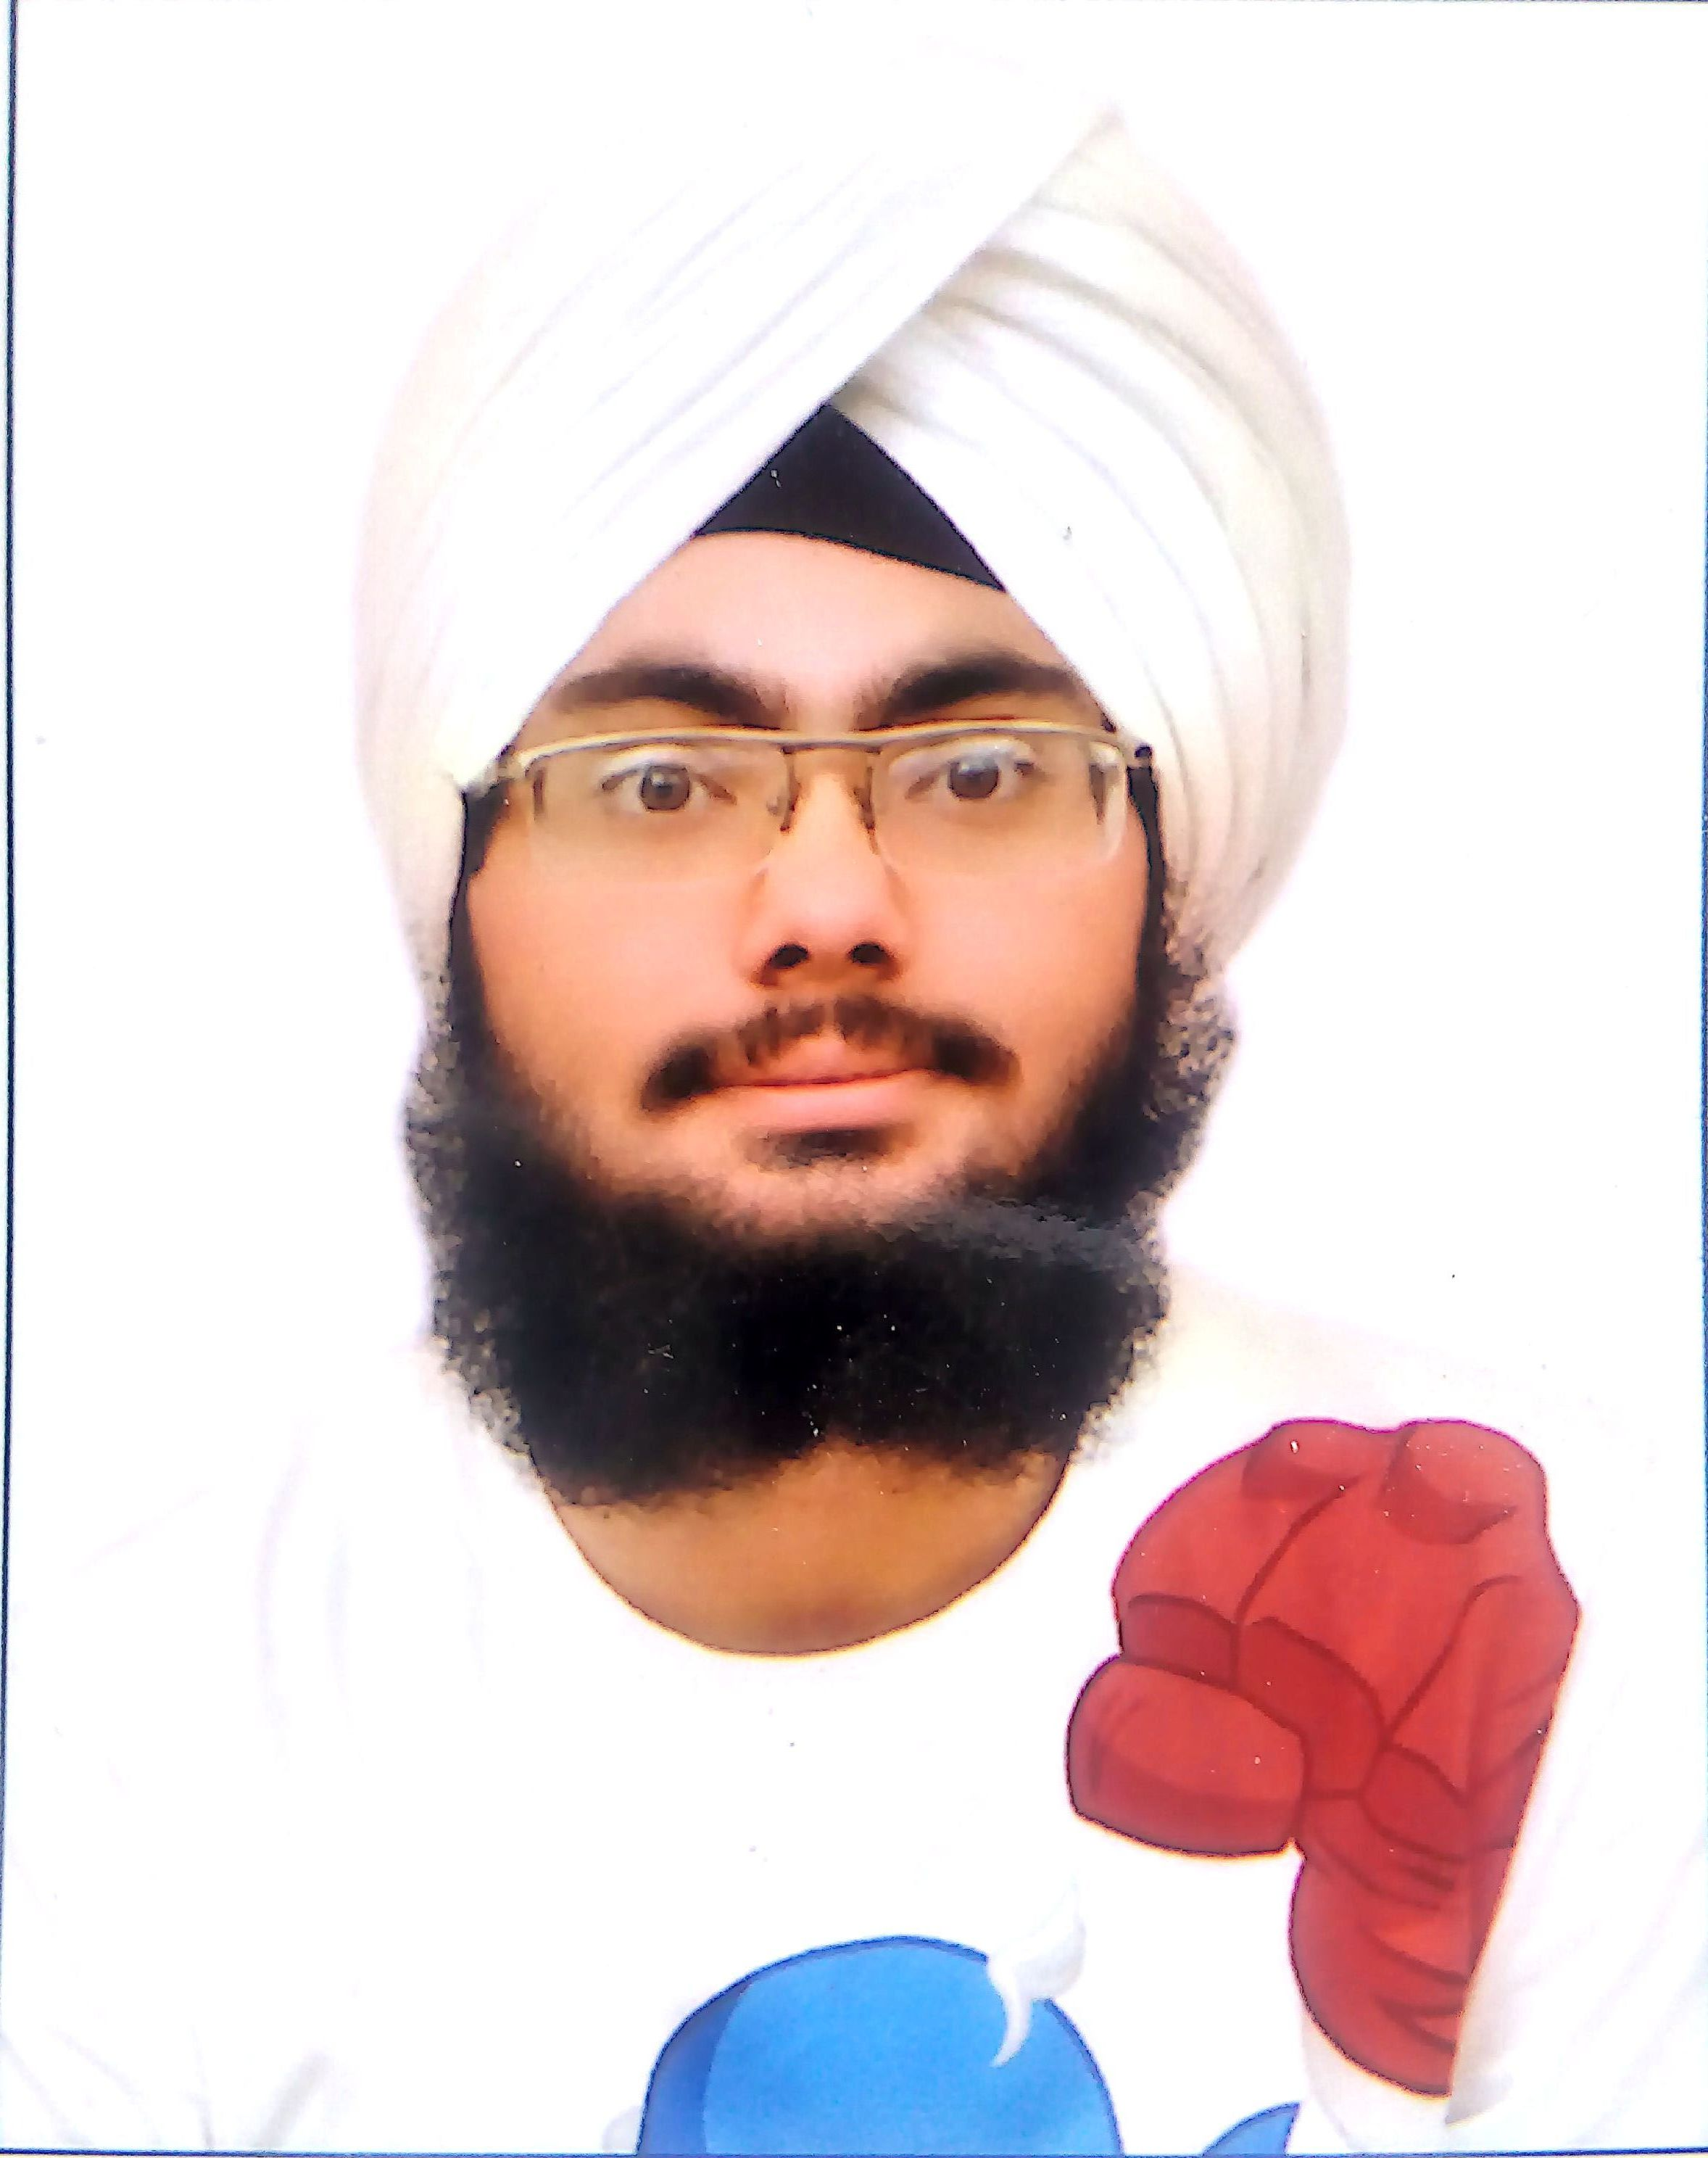
\includegraphics[width=2.5cm, height=3.5cm]{pic.jpg}	
\end{flushright}
\end{figure}



\begin{flushleft}
\textbf{OBJECTIVE }\\
\vskip  0.2cm
\hspace{0.2in}
To develop techincal skills
\end{flushleft}



\begin{flushleft}
\vspace{0.3in}
\textbf{EDUCATION }
\begin{center}
\begin{tabular}{| L{2cm} | C{4cm} | C{2cm} | C{2cm} | R{2cm}| }
\hline
Class & School & University & Passing Year & Passing percentage\\ 
\hline
10th & APJ Public School,Sheikh Sarai,New Delhi & CBSE & 2012 & CGPA 10.0\\
\hline
12th & Ambience Public School,Safdarjung Enclave,New Delhi & CBSE & 2014 & 94.6\% \\
\hline
\end{tabular}
\end{center}
\end{flushleft}



\begin{flushleft}
\textbf{Projects }
\begin{flushright}
\begin{enumerate}
\item "Gas Leakage Detection"Theme eY-RC 16
\end{enumerate} 
\end{flushright}
\end{flushleft}



\begin{flushleft}
\textbf{Training and Internship}
\begin{flushright}
\begin{itemize}
\item Attended workshop on 8051 conducted be RoboTryst
\end{itemize} 
\end{flushright}
\end{flushleft}


\begin{flushleft}
\textbf{Research Publications }
\end{flushleft}



\begin{flushleft}
\textbf{Technical Skills}
\begin{flushright}
\begin{itemize}
\item Knowledge of C
\item Knowledge of C++
\item Knowledge of embedded C
\item Knowledge of Matlab
\end{itemize} 
\end{flushright}
\end{flushleft}




\begin{flushleft}
\textbf{Soft Skills }
\begin{flushright}
\begin{enumerate}
\item Time Management
\item Resource Management
\item Leadership
\end{enumerate} 
\end{flushright}
\end{flushleft}



\begin{flushleft}
\textbf{Extracirricular Activites}
\begin{flushright}
\begin{itemize}
\item Playing Football
\item Playing badminton
\end{itemize} 
\end{flushright}
\end{flushleft}



\begin{flushleft}
\textbf{Co Cirricular activites }
\begin{flushright}
\begin{enumerate}
\item Member of IETE
\end{enumerate} 
\end{flushright}
\end{flushleft}



\begin{flushleft}
\textbf {Personal Details :  }
\vskip 0.2cm
\hspace{1.4in}
\begin{tabular}{ cc } 
 \hfill Fathers Name : & Parminder Pal Singh \\ 
 \hfill Mothers Name : & Parmjeet Kaur \\  
 \hfill Sex : & Male   \\ 
 \hfill Date Of Birth : & 06/09/1996  \\
 \hfill Nationality : & Indian  \\
 \hfill Marital Status : & Single
\end{tabular}
\end{flushleft}





\begin{flushleft}
\textbf{Reference}
\end{flushleft}

\vskip 0.3cm


\begin{flushleft}
\textbf{Declaration : }
 I hereby declare that the above written particulars are true to the best of my \\
\hspace{1in}
knowledge and belief.
\end{flushleft}



\end{document}